\section{Vanilla Diagnostic Performance and Censorship Analysis (Scenario 3)}
\label{sec:scenario3-results}

Scenario 3 established the diagnostic baseline for the experiment, evaluating the efficacy of a traditional RCA heuristic running against a Vanilla Kubernetes environment. In this scenario, the automated agent was constrained to standard \textit{log-scraping} methodologies, polling the \texttt{stdout/stderr} streams of the cluster pods using regex signature matching. The ground-truth faults consisted of a $2000\,\text{ms}$ network delay randomly injected into one of four critical microservices (\texttt{cart}, \texttt{currency}, \texttt{payment}, or \texttt{shipping}).

\subsection{Censorship Rate and Silent Degradation}

The empirical results from $N=30$ trials revealed a severe diagnostic limitation inherent to native log-based troubleshooting in microservices. As illustrated in Figure~\ref{fig:scenario3_outcomes}, the Vanilla agent suffered an overwhelming right-censorship rate of $80.00\%$ (24 out of 30 trials).

\begin{figure}[htbp]
    \centering
    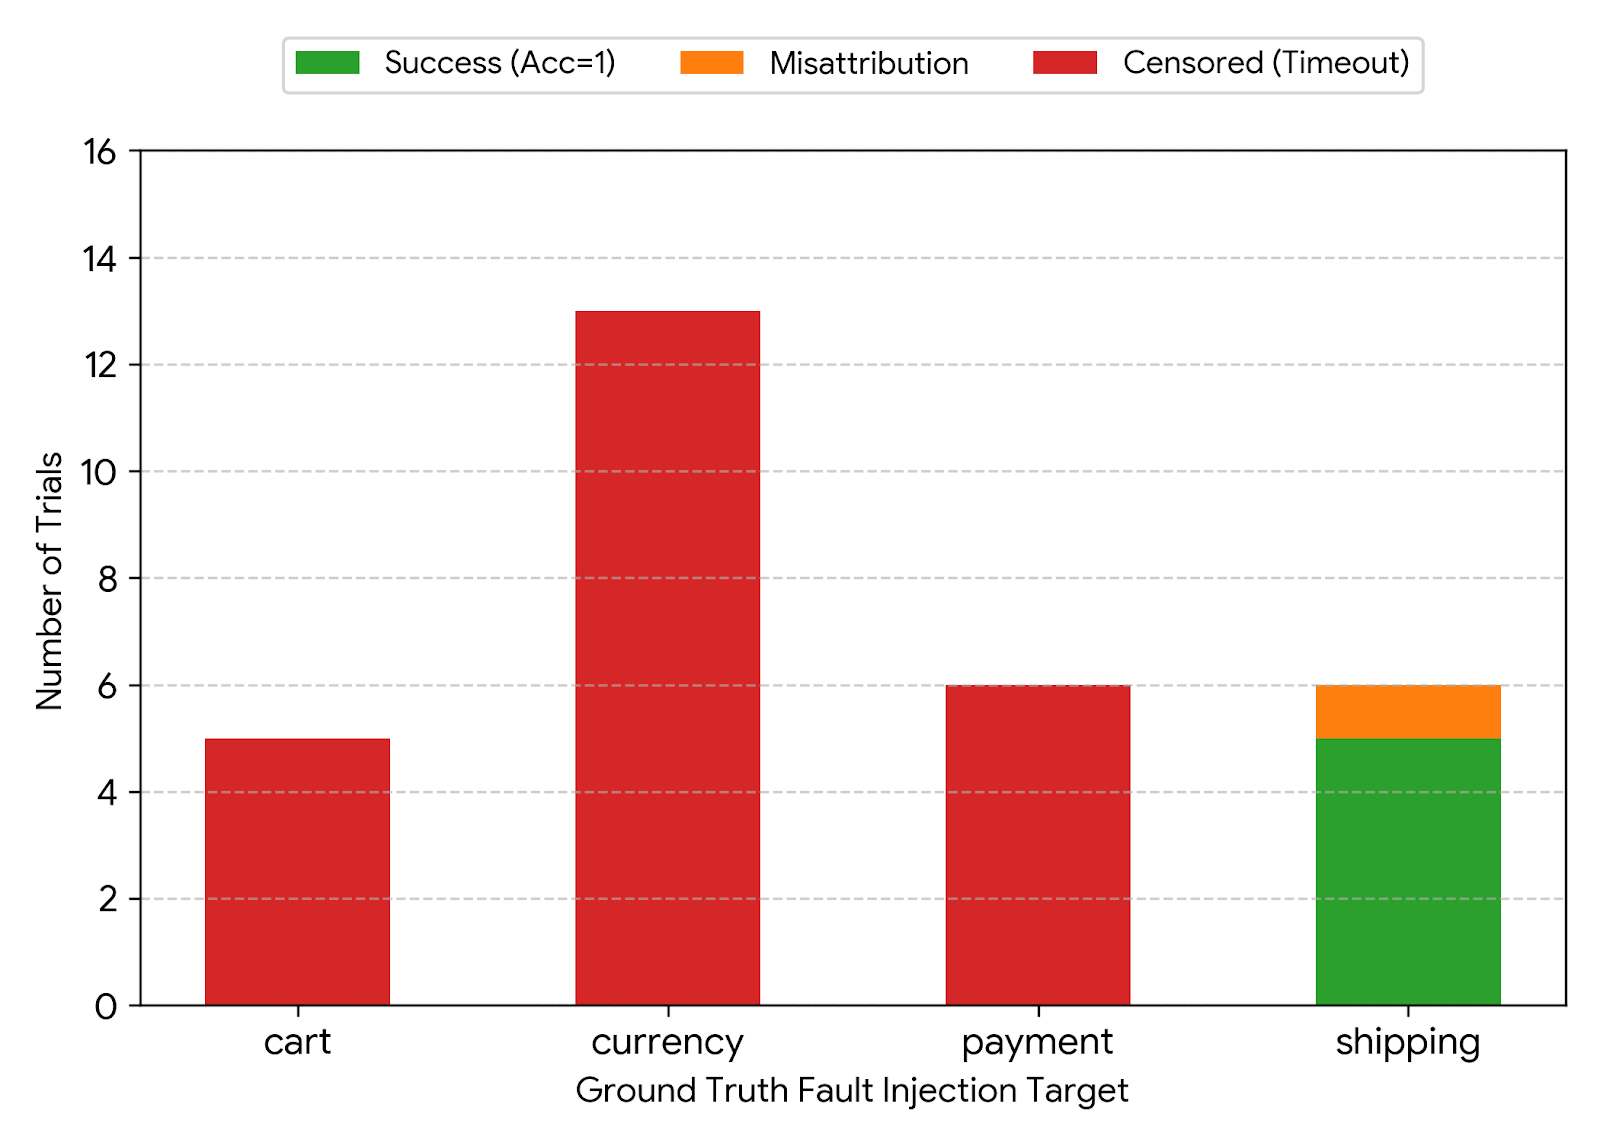
\includegraphics[width=0.85\textwidth]{images/results/scenario3_outcomes.png}
    \caption{Diagnostic outcomes of the Vanilla log-scraping agent grouped by the ground-truth fault injection target ($N=30$).}
    \label{fig:scenario3_outcomes}
\end{figure}

The high timeout rate is a direct manifestation of "silent" performance degradation. When network latency was injected into the \texttt{cart}, \texttt{currency}, or \texttt{payment} services, the components did not immediately crash or emit fatal stack traces. Instead, they experienced prolonged execution states that cascaded upstream as pure latency. Because standard log scraping relies on explicit error string emissions (e.g., \texttt{Exception}, \texttt{500 Internal Server Error}), the agent remained fundamentally blind to the underlying degradation, looping continuously until the 300-second timeout threshold was breached.

\subsection{Asymmetric Success and Protocol Boundaries}

The only diagnostic successes in Scenario 3 occurred when the fault was injected into the \texttt{shipping} service. Out of 6 trials targeting \texttt{shipping}, the agent correctly diagnosed the root cause in 5 instances ($Acc=1$) and misattributed it to the \texttt{frontend} in 1 instance.

This asymmetric success rate is explained by the protocol boundary behavior of the specific service. When the $2000\,\text{ms}$ delay was applied to \texttt{shipping}, the upstream HTTP client within the \texttt{frontend} service exceeded its hardcoded context deadline, abruptly aborting the connection. This forced the \texttt{frontend} pod to emit explicit connection failure logs (e.g., \textit{"failed POST to shipping service: EOF"}). The regex engine successfully captured this explicit signature, attributing the failure to the shipping module.

Ultimately, Scenario 3 demonstrates that RCA protocols reliant solely on unstructured application logs are structurally inadequate for modern cloud-native architectures. They perform adequately only when faults manifest as hard crashes or explicit protocol timeouts, failing completely to diagnose the cascading latency bottlenecks that characterize distributed microservice degradation.